\documentclass[beamer]{standalone}
\begin{document}

\title[Electronics 1] % (optional, use only with long paper titles)
{
	Alternating-Current Circuits
}

\begin{frame} 
  \titlepage
\end{frame}

\hide{
\begin{frame}
  \frametitle{Outline}
  \tableofcontents
  % You might wish to add the option [pausesections]
\end{frame}
}

\begin{frame}{Complex Number}
 \begin{block}{Out with $i$, in with $j$}
  Since $i$ will be reserved for currents, so complex numbers will be indicated with $j$ instead, with
  \begin{equation}
   j^2 = -1
  \end{equation}
 \end{block}
 \begin{block}{Properties of complex numbers, also covered in Physics 301}
  \begin{itemize}
   \item $\frac{1}{j} = \frac{j}{j^2} = \frac{j}{-1} = -j$
   \item $j = e^{j \pi/2}$ so $\frac{1}{j} = j^{-1} = e^{-j \pi/2}$
   \item $z = |z| e^{j \phi} = |z| \cos\phi + j |z| \sin\phi$
  \end{itemize}
 \end{block}
 \begin{block}{Physical meaning of complex numbers}
  We will use complex impedance $Z$ and complex gain $G(\omega)$ to indicate a phase shift of $\phi$
 \end{block}
\end{frame}

\section{Complex Impedances}
\begin{frame}
 \frametitle{Alternating-Current Signals}
 \begin{block}{Exponential notation}
  Consider voltage and current as real part of complex exponential:
  \begin{eqnarray*}
   v(t) & = & v_0 \cos(\omega t + \phi_v) = v_0 Re (e^{j (\omega t + \phi_v)}) \\
   i(t) & = & i_0 \cos(\omega t + \phi_i) = i_0 Re (e^{j (\omega t + \phi_i)})
  \end{eqnarray*}
  Now do all calculations in complex numbers.
 \end{block}
 \begin{block}{Resistors and Ohm's law: no phase difference}
  Resistance is given by
  \begin{equation*}
   R = \frac{v(t)}{i(t)} = \frac{v_0}{i_0} e^{j (\phi_v - \phi_i)}
  \end{equation*}
  but because $i(t)$ is always in phase with $v(t)$, we always have $(\phi_v - \phi_i) = 0$.
 \end{block}
\end{frame}

\begin{frame}
 \frametitle{Alternating-Current Signals}
 \begin{block}{Components with phase difference}
  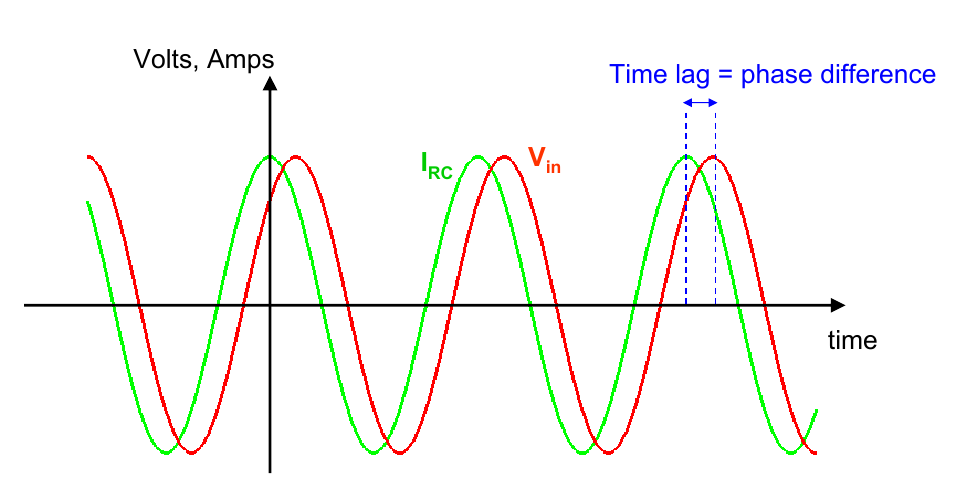
\includegraphics[width=\textwidth]{pics/Phase_difference} \\
  CIVIL: in capacitor I before V; V before I in inductor
 \end{block}
\end{frame}


\begin{frame}[t]
 \frametitle{Complex Impedances}
 \begin{block}{Impedance $Z$ of common components}
  \begin{center}
   \begin{tabular}{c|c|l|l}
    resistor & R & \\
    capacitor & $\frac{1}{j\omega C}$ & open for $\omega \to 0$ & short for $\omega \to \infty$ \\
    inductor & $j\omega L$ & short for $\omega \to 0$ & open for $\omega \to \infty$ \\
   \end{tabular}
  \end{center}
 \end{block}
 \only<2>{
 \begin{block}{Example: inductor}
  Start from differential equation describing inductor
  \begin{eqnarray*}
   v(t) & = & L \frac{d}{dt} i(t) = L \frac{d}{dt} Re(i_0 e^{j(\omega t + \phi_i)}) \\
        & = & Re(j \omega L i_0 e^{j(\omega t + \phi_i)})
  \end{eqnarray*}
  The impedance is then
  \begin{equation*}
   Z(\omega) = \frac{v(t)}{i(t)} = \frac{j \omega L i_0 e^{j(\omega t + \phi_i)}}{i_0 e^{j(\omega t + \phi_i)}} = j \omega L
  \end{equation*}
 \end{block}
 }
 \begin{block}{Impedances in series and in parallel}<3>
  \begin{itemize}
   \item In series: $Z = Z_1 + Z_2$
   \item In parallel: $\frac{1}{Z} = \frac{1}{Z_1} + \frac{1}{Z_2}$
   \item Because $Z \sim \frac{1}{C}$ this works for capacitors.
  \end{itemize}
 \end{block}
\end{frame}

\begin{frame}
 \frametitle{Complex Impedances}
 \begin{block}{Example: RLC circuit}
  \begin{center}
   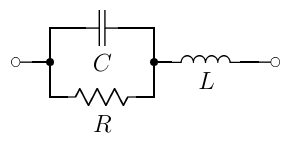
\includegraphics[width=0.4\textwidth]{pics/RLC_circuit}
  \end{center}
  \only<1>{What is the equivalent impedance $Z_{eq}$?}
 \end{block}
 \begin{block}<2->{Equivalent impedance}
  \begin{equation*}
   Z_{eq} = \frac{R}{j \omega R C + 1} + j \omega L
  \end{equation*}
  \only<2>{What are the limits for small and large $\omega$?}
 \end{block}
 \begin{block}<3->{Limits for small and large $\omega$}
  \begin{itemize}
   \item $\omega \approx 0$ (DC limit): $Z_{eq} \approx R$
   \item $\omega \to \infty$ (high frequency limit): $Z_{eq} \approx j\omega L$
  \end{itemize}
 \end{block}
\end{frame}


\section{Power Dissipation and Root-Mean-Square}
\begin{frame}
 \frametitle{Power Dissipation}
 \begin{block}{Power dissipation in resistor: root mean square}
  Dissipated power in a resistor is 
  \begin{equation*}
   P_{avg} = R \frac{1}{T} \int_{t=0}^T i(t)^2 dt = R I_{RMS}^2 = V_{RMS} I_{RMS}
  \end{equation*}
 \end{block}
 \begin{block}{Power dissipation in general impedance}
  \begin{equation*}
   P_{avg} = \frac{1}{T} \int_{t=0}^T v(t) \cdot i(t) dt
  \end{equation*}
  \begin{itemize}
   \item In phase (like a resistor): $P_{avg} = \frac{1}{2} v_0 i_0 = V_{RMS} I_{RMS}$
   \item $90^\circ$ out of phase (like a capacitor or inductor): $P_{avg} = 0$
   \item Anything in between: $Z = R + j X$, with reactance $X$
  \end{itemize}
 \end{block}
\end{frame}
\begin{frame}
 \frametitle{Power Dissipation}
 \begin{block}{Power factor}
  \begin{itemize}
   \item Dissipated power only depends on $R$
   \item Power company still has to generate $|Z|$
   \item Keep ratio ($\sim$ power factor) close to 1 with large capacitor banks
  \end{itemize}
 \end{block}
 \begin{center}
  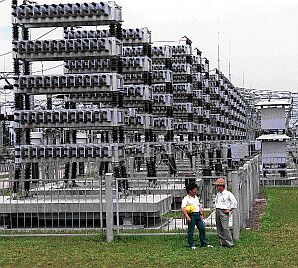
\includegraphics[width=0.45\textwidth]{pics/capacitor_bank}
 \end{center}
\end{frame}


\section{Transformers}
\begin{frame}
 \frametitle{Transformers}
 \begin{columns}
  \begin{column}{0.4\textwidth}
   \includegraphics<1>[width=\textwidth]{pics/transformers_prime}
   \includegraphics<2>[width=\textwidth]{pics/transformers} \\
   \only<2>{Flux $\Phi = \mu N_1 i_1(t) A$, where $A$ cross-sectional area, $N_1$ windings}
  \end{column}
  \begin{column}{0.6\textwidth}
   \begin{block}{Magnetic flux conserved}
    \begin{itemize}
     \item EMF $\mathcal{E}$ by $v_1(t)$ and $v_2(t)$ must be equal, so
      \begin{equation*}
       v_2 = \frac{N_2}{N_1} v_1
      \end{equation*}
     \item Energy conservation requires that $P_1 = P_2 = i(t) v(t)$, so
      \begin{equation*}
       i_2 = \frac{N_1}{N_2} i_1
      \end{equation*}
     \item If we connect a load $Z_L$ across terminals 2, $v_2 = i_2 Z_L$, and then
      \begin{equation*}
       Z_{eq} = \frac{v_1}{i_1} = \left(\frac{N_1}{N_2}\right)^2 Z_L
      \end{equation*}
    \end{itemize}
   \end{block}
  \end{column}
 \end{columns}
\end{frame}



\section{Gain of a Circuit}
\begin{frame}[t]
 \frametitle{Gain of a Circuit}
 \begin{block}{Input/output voltage}
  \begin{columns}
   \begin{column}{0.0\textwidth}
   \end{column}
   \begin{column}{0.35\textwidth}
    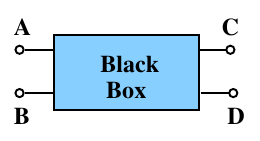
\includegraphics[width=\textwidth]{pics/Black_box}
   \end{column}
   \begin{column}{0.65\textwidth}
    \begin{itemize}
     \item Gain $G$ is $V_{CD} / V_{AB}$
     \item If $V_{CD}$ is 1.5\,V when $V_{AB}$ is 0.5\,V, \\ then the gain is 3.
    \end{itemize}
   \end{column}
  \end{columns}
 \end{block}
 \begin{block}{Gain of a DC voltage divider}
  \begin{columns}
   \begin{column}{0.0\textwidth}
   \end{column}
   \begin{column}{0.2\textwidth}
    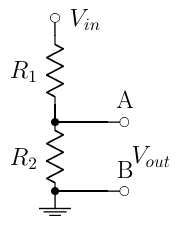
\includegraphics[width=\textwidth]{pics/Voltage_divider}
   \end{column}
   \begin{column}{0.8\textwidth}
    \begin{itemize}
     \item Voltage divider with two resistors: \\ input $V_{AB}$ is $V_{in}$, output $V_{CD}$ is $V_{out}$
     \item Gain $G$ is $V_{out} / V_{in} = \frac{R_2}{R_1 + R_2}$
     \item Now extend this concept to alternating-current signals\ldots
    \end{itemize}
   \end{column}
  \end{columns}
 \end{block}
\end{frame}

\begin{frame}[t]
 \frametitle{Gain of a Circuit}
 \begin{block}{Gain of a AC voltage divider}
  \begin{columns}
   \begin{column}{0.0\textwidth}
   \end{column}
   \begin{column}{0.5\textwidth}
    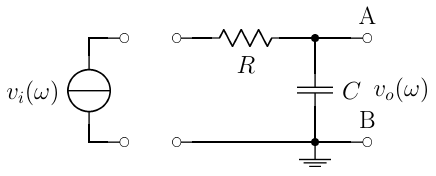
\includegraphics[width=\textwidth]{pics/RC_filter}
   \end{column}
   \begin{column}{0.5\textwidth}
    \begin{itemize}
     \item Gain $G(\omega)$ is now $v_o(\omega) / v_i(\omega) = \frac{Z_2(\omega)}{Z_1(\omega) + Z_2(\omega)}$
     \item $G(\omega)$ depends on frequency!
     \item $G(\omega)$ is a complex number!
    \end{itemize}
   \end{column}
  \end{columns}
 \end{block}
 \begin{columns}[t]
  \begin{column}{0.5\textwidth}
   \begin{block}{Impedances of RC-circuit}
    \begin{eqnarray*}
     Z_1 & = & R \\
     Z_2 & = & \frac{1}{j\omega C}
    \end{eqnarray*}
   \end{block}
  \end{column}
  \begin{column}{0.0\textwidth}
  \end{column}
  \begin{column}{0.5\textwidth}
   \begin{block}{Gain of this RC-circuit}
    \begin{eqnarray*}
     G(\omega) & = & \frac{1}{j\omega C} \frac{1}{R +\frac{1}{j\omega C}} \\
               & = & \frac{1}{1 + j\omega R C}
    \end{eqnarray*}
   \end{block}
  \end{column}
 \end{columns}
\end{frame}

\begin{frame}
 \frametitle{Gain of a Circuit}
 \begin{block}{Limits of gain in an RC-circuit}
  \begin{columns}
   \begin{column}{0.0\textwidth}
   \end{column}
   \begin{column}{0.5\textwidth}
    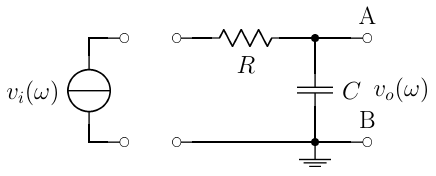
\includegraphics[width=\textwidth]{pics/RC_filter}
   \end{column}
   \begin{column}{0.5\textwidth}
    \begin{equation*}
     G(\omega) = \frac{1}{1 + j\omega R C}
    \end{equation*}
   \end{column}
  \end{columns}
  \begin{itemize}
   \item Low frequency $\omega \ll \frac{1}{RC}$: $G(\omega) \approx 1$ (DC limit)
   \item High frequency $\omega \gg \frac{1}{RC}$: $G(\omega) \approx \frac{1}{j\omega R C} \approx 0$
  \end{itemize}
 \end{block}
 \only<1>{
 \begin{block}{Bode plots}
  \begin{center}
   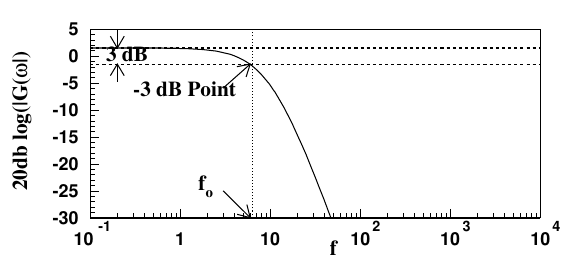
\includegraphics[width=0.4\textwidth]{pics/Bode_plot}
  \end{center}
 \end{block}
 }
 \only<2>{
 \begin{block}{Exercise: Swapping $R$ and $C$}
  \begin{itemize}
   \item How will the gain change when $R$ and $C$ are swapped?
   \item How will the Bode plot change?
  \end{itemize}
 \end{block}
 }
\end{frame}

\section{Power dissipation}
\begin{frame}
\frametitle{Power dissipation}
	Recall that power dissipated by element is
	\[P=V I\] where $V$ and $I$ are real.

	Since we use a  substitute \\
	$V\cos(\omega t) \to V e^{j \omega t}$ 
	and  $I\cos(\omega t) \to I e^{j \omega t}$,  \\
	we need to write
	\alert{
	\[P=Re(V) Re(I)\]
	}
	Recall the Ohm's law
	\[ V=Z I\]
\end{frame}

\begin{frame}
\frametitle{Power dissipation by a reactive element}
	\begin{theorem} 
		{\bf Average power dissipated by a reactive element (C or L) is 0} \\
		Lets use as example an inductor. \\
		\vskip -.1in
		\[Z_L=i \omega L = e^{i \frac{\pi}{2}} \omega L,
		 I_L= I_p e^{ i \omega t} \]
		\[V_L=Z_L I_L = e^{i \frac{\pi}{2}} \omega L I_L
		= \omega L I_p e^{ i (\omega t + \frac{\pi}{2} ) }  \]
		\[ Re(I_L)=I_p \cos(\omega t),  Re(V_L)= - \omega I_p L \sin(\omega t) \]
		Thus average power dissipated by the inductor
		\[P=\int^T_0 Re(I_L) Re(V_L) dt
		= - \int^T_0 I_p \cos(\omega t) \omega I_p L \sin(\omega t) dt \]
		\[P
		= - \omega I_p^2 L \int^T_0 \cos(\omega t) \sin(\omega t) dt 
		= \omega I_p^2 L \int^T_0 \frac{1}{2} \sin(2 \omega t) dt = 0\]
	\end{theorem}
\end{frame}

\end{document}
